\documentclass[11pt]{article}

\usepackage[margin=1in]{geometry}
\usepackage{amsmath,amssymb}
\usepackage{xcolor}
\usepackage{listings}
\usepackage{booktabs}
\usepackage{enumitem}
\usepackage{hyperref}
\usepackage{xspace}
\usepackage{tikz}
\usetikzlibrary{arrows.meta,positioning,shapes,fit,backgrounds,calc}

\lstdefinestyle{code}{
  basicstyle=\ttfamily\footnotesize,
  columns=fullflexible,
  keepspaces=true,
  breaklines=true,
  frame=single,
  numbers=none,
  showstringspaces=false,
}
\lstset{style=code}

% ---- palette: one colour per node tag ------------------------------------
\definecolor{fncol}{RGB}{200,120,20}    % FUNCTION_TAG  (unevaluated call)
\definecolor{fwcol}{RGB}{40,90,160}     % FORWARD_TAG
\definecolor{chcol}{RGB}{60,130,60}     % CHOICE_TAG
\definecolor{flcol}{RGB}{190,40,40}     % FAIL_TAG
\definecolor{cutcol}{RGB}{190,40,40}

\newcommand{\btomd}{\texttt{backtracking-\allowbreak optimizations.md}\xspace}
\newcommand{\code}[1]{\texttt{#1}}

% ---- TikZ styles ---------------------------------------------------------
\tikzset{
  cell/.style={draw, rounded corners=2pt, inner sep=3pt, minimum height=0.75cm,
    minimum width=1.25cm, align=center, font=\footnotesize},
  fn/.style={cell, draw=fncol, fill=fncol!12},
  fw/.style={cell, draw=fwcol, fill=fwcol!10},
  co/.style={cell, draw=black!70, fill=white},
  ch/.style={cell, draw=chcol, fill=chcol!13},
  fl/.style={cell, draw=flcol, fill=flcol!12},
  orph/.style={cell, dashed, draw=black!45, fill=black!4, text=black!55},
  ptr/.style={-{Stealth[length=4pt,width=3pt]}, semithick},
  fptr/.style={-{Stealth[length=4pt,width=3pt]}, very thick, draw=fwcol},
  gone/.style={-{Stealth[length=4pt,width=3pt]}, semithick, dashed, draw=black!40},
  drv/.style={draw=none, font=\footnotesize\itshape, inner sep=1pt},
  badge/.style={font=\tiny\bfseries, text=red!70!black, inner sep=1pt},
  note/.style={font=\scriptsize, text=black!70, align=left},
  alarm/.style={font=\scriptsize\bfseries, text=red!70!black, align=left, text width=3.2cm},
  trail/.style={draw=black!60, rounded corners=2pt, fill=black!3, inner sep=4pt,
    anchor=north west, font=\scriptsize},
}

% node label: cell name (italic, small) over its contents (typewriter)
\newcommand{\cn}[2]{{\scriptsize\itshape #1}\\[-1pt]{\ttfamily #2}}

% trail rows: frame name, cell, pre-image, flag
\newcommand{\fr}[4]{\textbf{#1} & #2 & $\mapsto$ & \texttt{#3} & #4\\}
\newcommand{\dead}[4]{\textcolor{black!45}{\textbf{#1}} & \textcolor{black!45}{#2} &
  \textcolor{black!45}{$\mapsto$} & \textcolor{black!45}{\texttt{#3}} &
  \textcolor{black!45}{\textit{(popped)}}\\}
\newcommand{\cutrow}[1]{\hline\multicolumn{5}{@{}l@{}}{\textcolor{cutcol}{\textbf{#1}}}\\\hline}
\newcommand{\trailnode}[2]{\node[trail] at (#1) {%
  \begin{tabular}{@{}l@{\;}l@{\;}c@{\;}l@{\;}l@{}}
  \multicolumn{5}{@{}l@{}}{\itshape trail (top of stack first)}\\ #2 \hline
  \end{tabular}};}

\title{Where Scoped Retry Goes Wrong:\\
Heap and Trail Graphs for Two Failing Programs}
\author{Rice project notes}
\date{}

\begin{document}
\maketitle

\begin{abstract}
\btomd's optimization \#3 (scoped backtracking), generalized so that every
generated \code{\_hnf} function calls \code{SCOPED\_CUTOFF()} on entry and
\code{SCOPED\_RETRY(...)} on a failing case, silently gives wrong answers on
real programs. This note draws the heap graph and the backtracking trail,
step by step, for two small programs that expose it, and pins the failures on
two independent defects. Both are the same kind of mistake: after a scoped
\code{undo}, the trail no longer contains a record for every heap cell that
has been overwritten since the choice point it is supposed to protect. Sharing
enters in two ways: graph reduction overwrites \emph{shared} cells in place
(which is the only reason there is a trail at all), and in the first example
a \emph{shared choice} ties a failure deep inside one case to a decision made
by another. A third ingredient, control passing along heap edges instead of
the C stack, is what makes a stack-height cutoff the wrong notion of scope in
the second. Experiments with both defects patched in scratch
copies produce correct output on all three programs tried; that shows the
defects are sufficient to explain these failures, not that the optimization is
now sound (Section~\ref{sec:summary}).
\end{abstract}

%% ==========================================================================
\section{Reading the figures}
%% ==========================================================================

\subsection{What the runtime does, in four sentences}

\begin{enumerate}[nosep]
\item \textbf{Evaluation overwrites cells in place.} Reducing a node
  replaces its contents with its result (a forward to another cell, a
  constructor, \code{FAIL}). Every parent that shares the node sees the
  result. This is what makes evaluation lazy \emph{and} shared.
\item \textbf{The trail is a log of those overwrites.} A frame is a pair
  $\text{cell}\mapsto\text{pre-image}$, plus a \emph{choice} bit.
  \code{choose} pushes a frame for the choice cell (choice bit set if
  another alternative remains); \code{save\_copy(root)} pushes one for a
  node about to be overwritten, but only when the node's \code{nondet} flag
  says it depended on some choice.
\item \textbf{\code{undo(c)} pops frames, restoring each cell, until it pops a
  choice frame or the stack height reaches $c$.} It returns whether it
  stopped on a choice frame. Global backtracking is \code{undo(0)}.
\item \textbf{Scoped retry} records \code{\_cutoff = size(bt\_stack)} when a
  generated function starts. When a case fails it calls
  \code{undo(\_cutoff)}: ``retry against any choice made \emph{since I
  started}.'' The assumption is that the frames above \code{\_cutoff} are
  exactly the overwrites made on behalf of this function's own computation.
\end{enumerate}

The relevant code (\code{runtime/runtime.c}, \code{runtime/runtime.h}):

\begin{lstlisting}[language=C]
#define SCOPED_CUTOFF()  int _cutoff = size(bt_stack)
#define SCOPED_RETRY(scrutinee_var, orig_var) \
  if (undo(_cutoff)) { scrutinee_var = orig_var; continue; }

bool undo(int cutoff) {
    if(bt_stack->size == 0) return false;
    FieldPair* frame;
    do {                                        // always pops at least once
        frame = pop(bt_stack);
        if(frame->lhs.n != NULL) memcpy(frame->lhs.n, frame->rhs.n, sizeof(Node));
    } while(!frame->choice && size(bt_stack) > cutoff);
    return frame->choice;
}
\end{lstlisting}

\subsection{Notation}

\begin{figure}[htb]
\centering
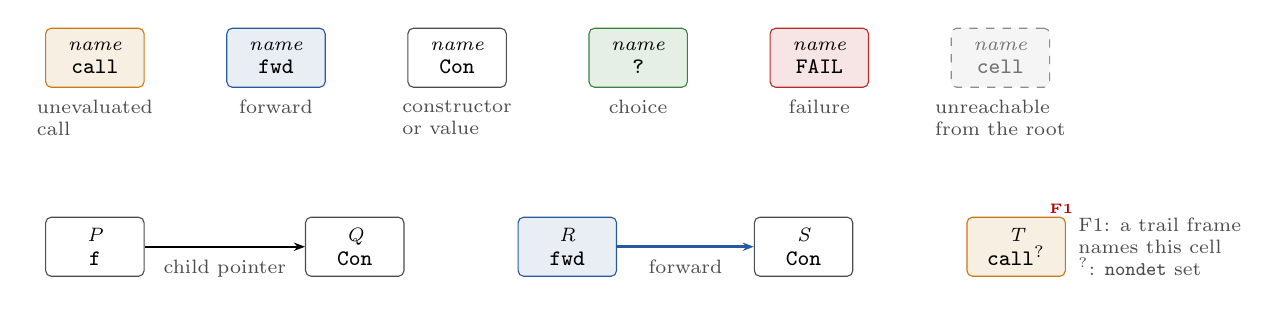
\begin{tikzpicture}
  \node[fn]  (a) at (0,0)   {\cn{name}{call}};
  \node[fw]  (b) at (2.3,0) {\cn{name}{fwd}};
  \node[co]  (c) at (4.6,0) {\cn{name}{Con}};
  \node[ch]  (d) at (6.9,0) {\cn{name}{?}};
  \node[fl]  (e) at (9.2,0) {\cn{name}{FAIL}};
  \node[orph](f) at (11.5,0){\cn{name}{cell}};
  \node[note, below=1pt of a] {unevaluated\\call};
  \node[note, below=1pt of b] {forward};
  \node[note, below=1pt of c] {constructor\\or value};
  \node[note, below=1pt of d] {choice};
  \node[note, below=1pt of e] {failure};
  \node[note, below=1pt of f] {unreachable\\from the root};
  \node[co] (p) at (0,-2.4) {\cn{P}{f}};
  \node[co] (q) at (3.3,-2.4) {\cn{Q}{Con}};
  \draw[ptr] (p) -- node[note, below=1pt] {child pointer} (q);
  \node[fw] (r) at (6.0,-2.4) {\cn{R}{fwd}};
  \node[co] (s) at (9.0,-2.4) {\cn{S}{Con}};
  \draw[fptr] (r) -- node[note, below=1pt] {forward} (s);
  \node[fn, label={[badge]above right:F1}] (t) at (11.7,-2.4) {\cn{T}{call$^?$}};
  \node[note, right=1pt of t] {F1: a trail frame\\names this cell\\$^?$: \code{nondet} set};
\end{tikzpicture}
\caption{Cell colours and marks. Children are drawn left to right in source
  order (Rice's debug printer prints them right to left; the traces the
  figures were taken from are reversed accordingly).}
\label{fig:legend}
\end{figure}

A cell that has been overwritten \emph{loses its old children}: after
\code{save\_copy} and a rewrite the only remaining reference to the old form
is the trail frame's pre-image, which is written inside the trail box, not
drawn as a heap edge. Trail frames are named \textbf{F0}, \textbf{F1},
\ldots{} (bottom to top, in the order pushed), and a red rule in the trail
box marks the \code{\_cutoff} of the function about to call \code{undo}:
\emph{everything above the rule is in that function's scope}.

%% ==========================================================================
\section{Example 1: a shared choice, and a lost solution}\label{sec:ex1}
%% ==========================================================================

\begin{lstlisting}[language=Haskell]
g :: Bool -> Bool
g True  = failed
g False = False

f :: Bool -> Bool -> Int
f True  y = case y of False -> 1
f False y = case y of False -> 2

main :: Int
main = let c = True ? False in f c (g c)
\end{lstlisting}

The choice \code{c} is used twice: as the scrutinee of \code{f}, and inside
the argument \code{g c}. The two uses must agree. The only consistent
solution is \code{c = False}: then \code{g c = False} and \code{f False False
= 2}. With \code{c = True}, \code{g c} fails. Scoped retry off gives
\code{FAIL, 2}; the default build gives \code{FAIL, FAIL}, i.e.\ the solution
is lost.

After inlining, the compiler produces one cell per call. I call them
\textbf{F} (\code{main\_CASE5}, the outer case of \code{f}) and \textbf{G}
(\code{main\_CASE3}, the body of \code{g c}); the True branch of \code{f} is
\code{main\_CASE7}. Each case branch is its own C function with its own
\code{\_cutoff}.

\begin{figure}[p]
\centering
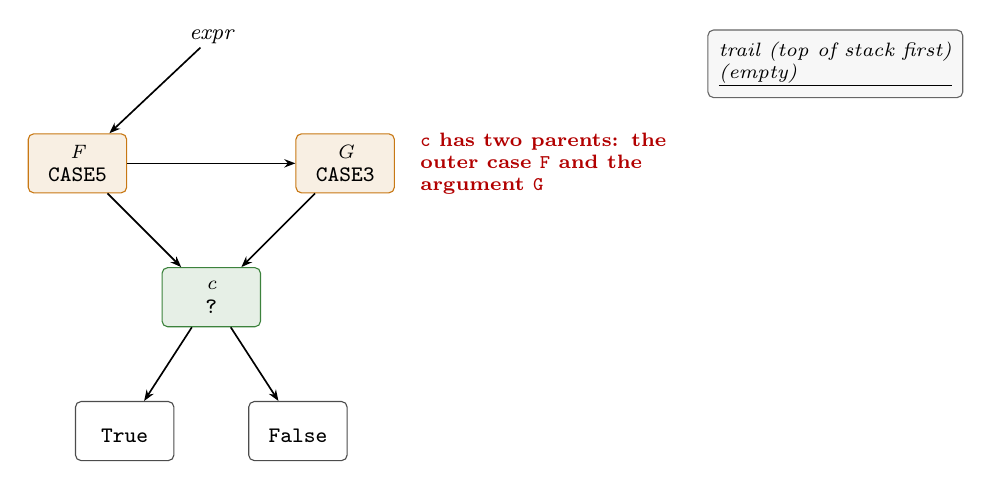
\begin{tikzpicture}
  \node[drv] (x) at (1.7,3.5) {expr};
  \node[fn] (F) at (0,1.9)  {\cn{F}{CASE5}};
  \node[fn] (G) at (3.4,1.9) {\cn{G}{CASE3}};
  \node[ch] (c) at (1.7,0.2) {\cn{c}{?}};
  \node[co] (T) at (0.6,-1.5) {\cn{}{True}};
  \node[co] (Fa) at (2.8,-1.5) {\cn{}{False}};
  \draw[ptr] (x) -- (F);
  \draw[ptr] (F) -- (c);
  \draw[ptr] (F) -- (G);
  \draw[ptr] (G) -- (c);
  \draw[ptr] (c) -- (T);
  \draw[ptr] (c) -- (Fa);
  \node[alarm, right=0.2 of G] {\code{c} has two parents: the outer case \code{F} and the argument \code{G}};
  \trailnode{8.0,3.6}{\multicolumn{5}{@{}l@{}}{\textit{(empty)}}\\}
\end{tikzpicture}
\caption{Before anything is evaluated. \code{F = f c G}, \code{G = g c}, and
  both share the choice cell \code{c}. (\code{c} is really a let-thunk that
  becomes this choice node when first forced; shown already forced.)}
\label{fig:b0}
\end{figure}

\begin{figure}[p]
\centering
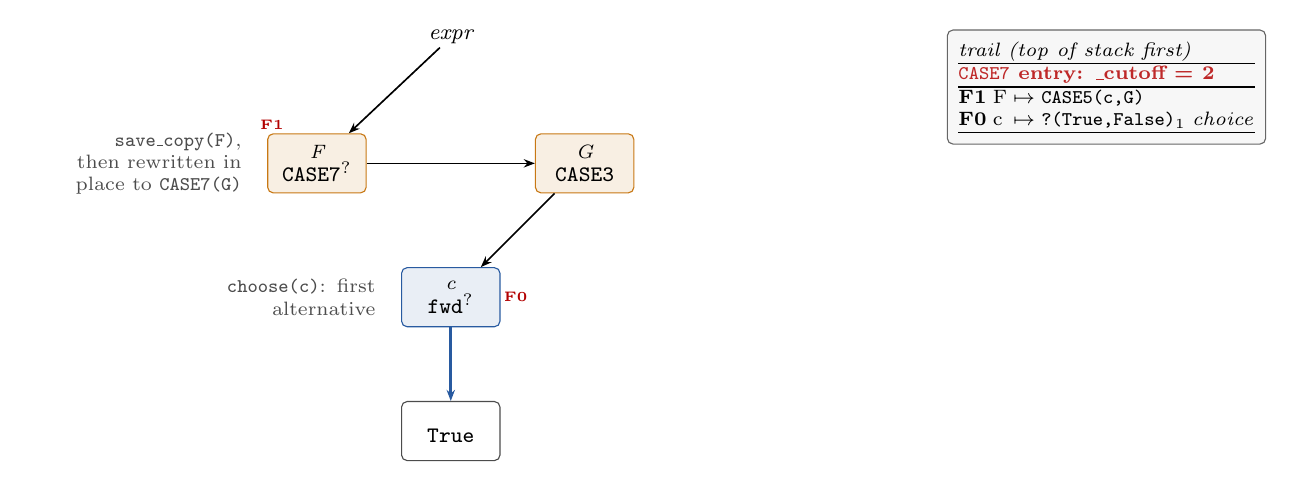
\begin{tikzpicture}
  \node[drv] (x) at (1.7,3.5) {expr};
  \node[fn, label={[badge]above left:F1}] (F) at (0,1.9)  {\cn{F}{CASE7$^?$}};
  \node[fn] (G) at (3.4,1.9) {\cn{G}{CASE3}};
  \node[fw, label={[badge]right:F0}] (c) at (1.7,0.2) {\cn{c}{fwd$^?$}};
  \node[co] (T) at (1.7,-1.5) {\cn{}{True}};
  \draw[ptr] (x) -- (F);
  \draw[ptr] (F) -- (G);
  \draw[ptr] (G) -- (c);
  \draw[fptr] (c) -- (T);
  \node[note, left=0.2 of c, align=right, text width=2.2cm] {\code{choose(c)}: first alternative};
  \node[note, left=0.2 of F, align=right, text width=2.6cm] {\code{save\_copy(F)}, then rewritten in place to \code{CASE7(G)}};
  \trailnode{8.0,3.6}{%
    \cutrow{\code{CASE7} entry: \_cutoff = 2}
    \fr{F1}{F}{CASE5(c,G)}{}
    \fr{F0}{c}{?(True,False)$_1$}{\textit{choice}}}
\end{tikzpicture}
\caption{\code{f}'s outer case dispatches on \code{c}. \code{F0} is the
  choice frame (\code{c}'s other alternative is still pending). \code{F}
  is then overwritten in place: it forgets \code{c} and now holds only
  \code{G}. \code{F1} is its old form. \code{CASE7}, the True branch of
  \code{f}, starts with \code{\_cutoff = 2}.}
\label{fig:b1}
\end{figure}

\begin{figure}[p]
\centering
\textbf{(i) \code{CASE3} (= \code{G}) reaches \code{g True = failed}, just before \code{undo(2)}.}\par\smallskip
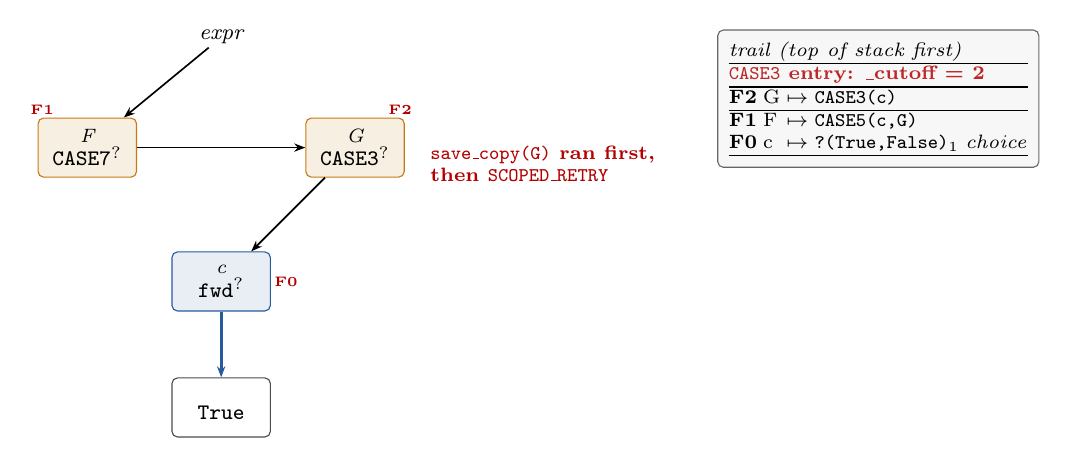
\begin{tikzpicture}
  \node[drv] (x) at (1.7,3.3) {expr};
  \node[fn, label={[badge]above left:F1}] (F) at (0,1.9)  {\cn{F}{CASE7$^?$}};
  \node[fn, label={[badge]above right:F2}] (G) at (3.4,1.9) {\cn{G}{CASE3$^?$}};
  \node[fw, label={[badge]right:F0}] (c) at (1.7,0.2) {\cn{c}{fwd$^?$}};
  \node[co] (T) at (1.7,-1.4) {\cn{}{True}};
  \draw[ptr] (x) -- (F);
  \draw[ptr] (F) -- (G);
  \draw[ptr] (G) -- (c);
  \draw[fptr] (c) -- (T);
  \node[alarm, right=0.2 of G, yshift=-0.2cm] {\code{save\_copy(G)} ran first, then \code{SCOPED\_RETRY}};
  \trailnode{8.0,3.4}{%
    \cutrow{\code{CASE3} entry: \_cutoff = 2}
    \fr{F2}{G}{CASE3(c)}{}
    \hline
    \fr{F1}{F}{CASE5(c,G)}{}
    \fr{F0}{c}{?(True,False)$_1$}{\textit{choice}}}
\end{tikzpicture}

\bigskip
\textbf{(ii) after \code{undo(2)} returned \emph{false} and \code{fail(G)} ran.}\par\smallskip
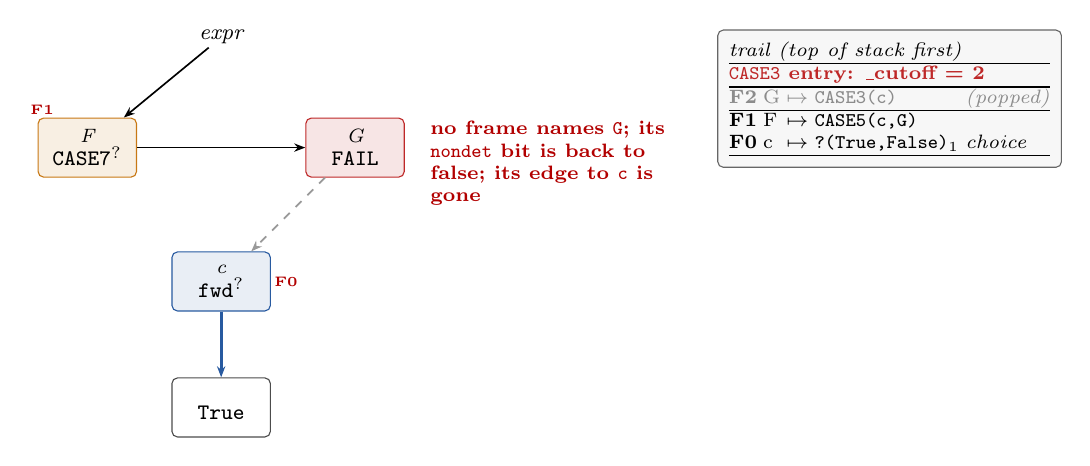
\begin{tikzpicture}
  \node[drv] (x) at (1.7,3.3) {expr};
  \node[fn, label={[badge]above left:F1}] (F) at (0,1.9)  {\cn{F}{CASE7$^?$}};
  \node[fl] (G) at (3.4,1.9) {\cn{G}{FAIL}};
  \node[fw, label={[badge]right:F0}] (c) at (1.7,0.2) {\cn{c}{fwd$^?$}};
  \node[co] (T) at (1.7,-1.4) {\cn{}{True}};
  \draw[ptr] (x) -- (F);
  \draw[ptr] (F) -- (G);
  \draw[fptr] (c) -- (T);
  \draw[gone] (G) -- (c);
  \node[alarm, right=0.2 of G, yshift=-0.2cm] {no frame names \code{G}; its \code{nondet} bit is back to false; its edge to \code{c} is gone};
  \trailnode{8.0,3.4}{%
    \cutrow{\code{CASE3} entry: \_cutoff = 2}
    \dead{F2}{G}{CASE3(c)}{}
    \hline
    \fr{F1}{F}{CASE5(c,G)}{}
    \fr{F0}{c}{?(True,False)$_1$}{\textit{choice}}}
\end{tikzpicture}
\caption{Defect 2. \code{showConsBranch} emits \code{save\_copy(root)} as the
  first thing in a constructor branch, so by the time the branch body
  reaches an unhandled case (\code{IExempt}) and calls \code{SCOPED\_RETRY},
  the scope already contains the frame \code{F2} that \code{save\_copy} just
  pushed. \code{undo(2)} finds no choice frame, so it returns false, but only
  after popping \code{F2}: \code{G} is restored to its raw form and the
  frame is gone. The next line, \code{fail(G)}, then overwrites \code{G}
  with no trail record at all. Restoring \code{G} also cleared its
  \code{nondet} bit (the pre-image was saved before the bit was set), so
  nothing downstream can tell this \code{FAIL} came from a choice.
  (The \code{FAIL\_TAG} path is emitted in the correct order: retry first,
  \emph{then} \code{save\_copy}, then \code{fail}.)}
\label{fig:b2}
\end{figure}

\begin{figure}[p]
\centering
\textbf{(i) \code{CASE7} sees its scrutinee \code{G} is \code{FAIL} and calls \code{undo(2)}.}\par\smallskip
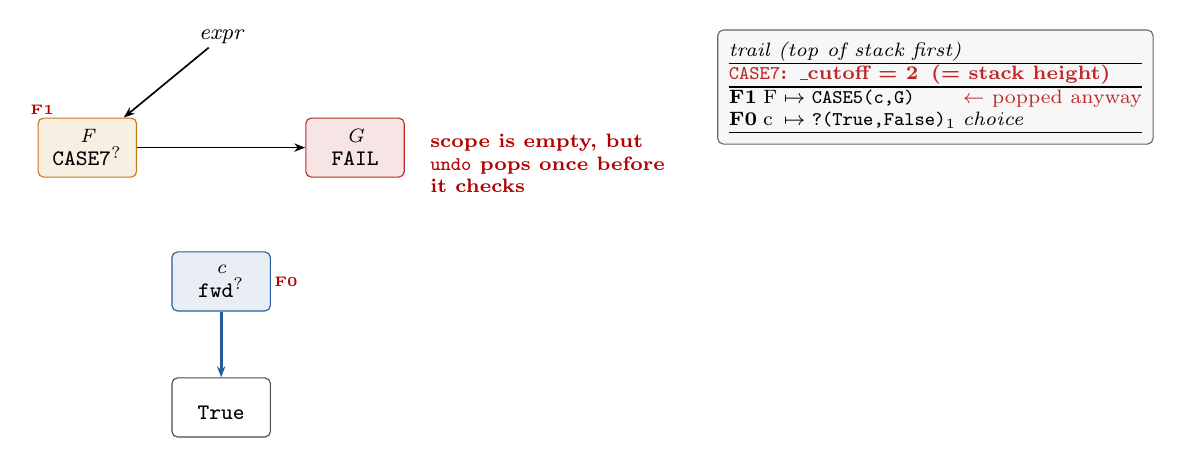
\begin{tikzpicture}
  \node[drv] (x) at (1.7,3.3) {expr};
  \node[fn, label={[badge]above left:F1}] (F) at (0,1.9)  {\cn{F}{CASE7$^?$}};
  \node[fl] (G) at (3.4,1.9) {\cn{G}{FAIL}};
  \node[fw, label={[badge]right:F0}] (c) at (1.7,0.2) {\cn{c}{fwd$^?$}};
  \node[co] (T) at (1.7,-1.4) {\cn{}{True}};
  \draw[ptr] (x) -- (F);
  \draw[ptr] (F) -- (G);
  \draw[fptr] (c) -- (T);
  \node[alarm, right=0.2 of G, yshift=-0.2cm] {scope is empty, but \code{undo} pops once before it checks};
  \trailnode{8.0,3.4}{%
    \cutrow{\code{CASE7}: \_cutoff = 2 \,(= stack height)}
    \fr{F1}{F}{CASE5(c,G)}{\textcolor{cutcol}{$\leftarrow$ popped anyway}}
    \fr{F0}{c}{?(True,False)$_1$}{\textit{choice}}}
\end{tikzpicture}

\bigskip
\textbf{(ii) after \code{undo(2)} returned \emph{false} and \code{fail(F)} ran.}\par\smallskip
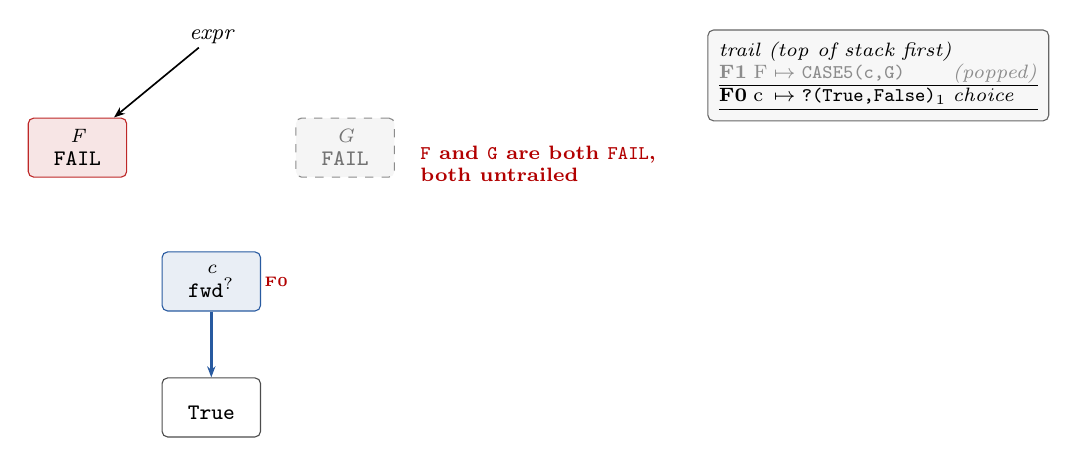
\begin{tikzpicture}
  \node[drv] (x) at (1.7,3.3) {expr};
  \node[fl] (F) at (0,1.9)  {\cn{F}{FAIL}};
  \node[orph] (G) at (3.4,1.9) {\cn{G}{FAIL}};
  \node[fw, label={[badge]right:F0}] (c) at (1.7,0.2) {\cn{c}{fwd$^?$}};
  \node[co] (T) at (1.7,-1.4) {\cn{}{True}};
  \draw[ptr] (x) -- (F);
  \draw[fptr] (c) -- (T);
  \node[alarm, right=0.2 of G, yshift=-0.2cm] {\code{F} and \code{G} are both \code{FAIL}, both untrailed};
  \trailnode{8.0,3.4}{%
    \dead{F1}{F}{CASE5(c,G)}{}
    \hline
    \fr{F0}{c}{?(True,False)$_1$}{\textit{choice}}}
\end{tikzpicture}
\caption{Defect 1. \code{CASE7}'s scope is empty: \code{F1} was pushed by
  \code{CASE5} \emph{before} it dispatched into \code{CASE7}, so it sits
  below \code{CASE7}'s cutoff. But \code{undo} is a \code{do}/\code{while}
  and always pops at least one frame, so it pops \code{F1} and restores
  \code{F} to \code{CASE5(c,G)}. Then \code{fail(F)} overwrites \code{F} with
  \code{FAIL}; because \code{G}'s \code{nondet} bit was lost in
  Figure~\ref{fig:b2}, \code{CASE7}'s own \code{nondet} is false and it does
  not re-save \code{F}. (Had the popped frame been a \emph{choice} frame,
  \code{undo} would have returned true, and a callee would have flipped a
  choice belonging to its ancestor.)}
\label{fig:b3}
\end{figure}

\begin{figure}[p]
\centering
\textbf{(i) scoped retry \emph{on}: the driver backtracks with \code{undo(0)}.}\par\smallskip
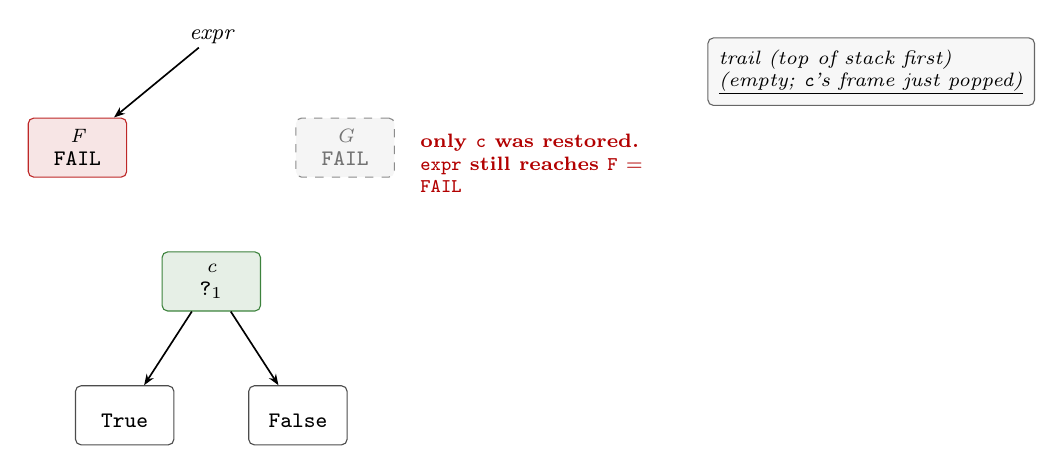
\begin{tikzpicture}
  \node[drv] (x) at (1.7,3.3) {expr};
  \node[fl] (F) at (0,1.9)  {\cn{F}{FAIL}};
  \node[orph] (G) at (3.4,1.9) {\cn{G}{FAIL}};
  \node[ch] (c) at (1.7,0.2) {\cn{c}{?$_1$}};
  \node[co] (T) at (0.6,-1.5) {\cn{}{True}};
  \node[co] (Fa) at (2.8,-1.5) {\cn{}{False}};
  \draw[ptr] (x) -- (F);
  \draw[ptr] (c) -- (T);
  \draw[ptr] (c) -- (Fa);
  \node[alarm, right=0.2 of G, yshift=-0.2cm] {only \code{c} was restored. \code{expr} still reaches \code{F} $=$ \code{FAIL}};
  \trailnode{8.0,3.3}{\multicolumn{5}{@{}l@{}}{\textit{(empty; \code{c}'s frame just popped)}}\\}
\end{tikzpicture}

\bigskip
\textbf{(ii) scoped retry \emph{off} (reference): the same point after \code{undo(0)}.}\par\smallskip
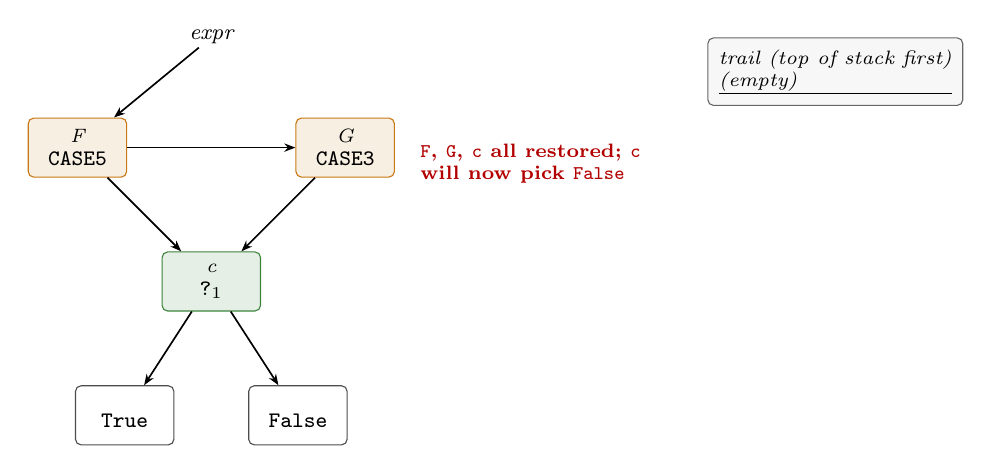
\begin{tikzpicture}
  \node[drv] (x) at (1.7,3.3) {expr};
  \node[fn] (F) at (0,1.9)  {\cn{F}{CASE5}};
  \node[fn] (G) at (3.4,1.9) {\cn{G}{CASE3}};
  \node[ch] (c) at (1.7,0.2) {\cn{c}{?$_1$}};
  \node[co] (T) at (0.6,-1.5) {\cn{}{True}};
  \node[co] (Fa) at (2.8,-1.5) {\cn{}{False}};
  \draw[ptr] (x) -- (F);
  \draw[ptr] (F) -- (c);
  \draw[ptr] (F) -- (G);
  \draw[ptr] (G) -- (c);
  \draw[ptr] (c) -- (T);
  \draw[ptr] (c) -- (Fa);
  \node[alarm, right=0.2 of G, yshift=-0.2cm] {\code{F}, \code{G}, \code{c} all restored; \code{c} will now pick \code{False}};
  \trailnode{8.0,3.3}{\multicolumn{5}{@{}l@{}}{\textit{(empty)}}\\}
\end{tikzpicture}
\caption{The consequence. (i) shows Figure~\ref{fig:b0} minus \code{F} and
  \code{G}: only the cell with a trail frame (\code{c}) is restored. The
  driver re-normalizes \code{expr}, follows it to \code{F}, and finds
  \code{FAIL} without ever re-evaluating anything, so \code{c = False} is
  never tried. (ii) is what backtracking must produce. With scoped retry off
  the trail at failure time was, top first: \code{F ${\mapsto}$ CASE7(G)},
  \code{G ${\mapsto}$ CASE3(c)}, \code{F ${\mapsto}$ CASE5(c,G)},
  \code{c ${\mapsto}$ ?} (choice); popping all four restores all three
  cells, and the shared choice \code{c} is set to flip. The next run takes
  \code{c = False}, \code{g False = False}, \code{f False False = 2}.}
\label{fig:b4}
\end{figure}

%% ==========================================================================
\section{Example 2: control passes through a heap edge}\label{sec:ex2}
%% ==========================================================================

This is the program from \code{debug\_repros/cent\_tiny.curry}: \code{eval
(mkExp2 3 0)}, where \code{mkExp2} builds a chain of four alternatives
\code{e1 :+ e2 ? e1 :- e2 ? e1 :* e2 ? e1 :/ e2} and \code{eval (x :/ y)} has
an incomplete \code{case} (no \code{False} branch when \code{y' > 0 \&\&
cond} is false). Only the last alternative, \code{3 :/ 0}, fails. With
scoped retry off the run prints \code{3, 3, 0, FAIL}; the default build
prints \code{3, 3, 0} and then the raw, unevaluated
\code{eval(:/(Num(0), Num(3)))}. (That is \code{eval (Num 3 :/ Num 0)}; the
debug printer lists children right to left.)

Here the failure happens inside a \emph{different function} from the one that
made the choice, and nothing on the C stack connects them.

\begin{figure}[htbp]
\centering
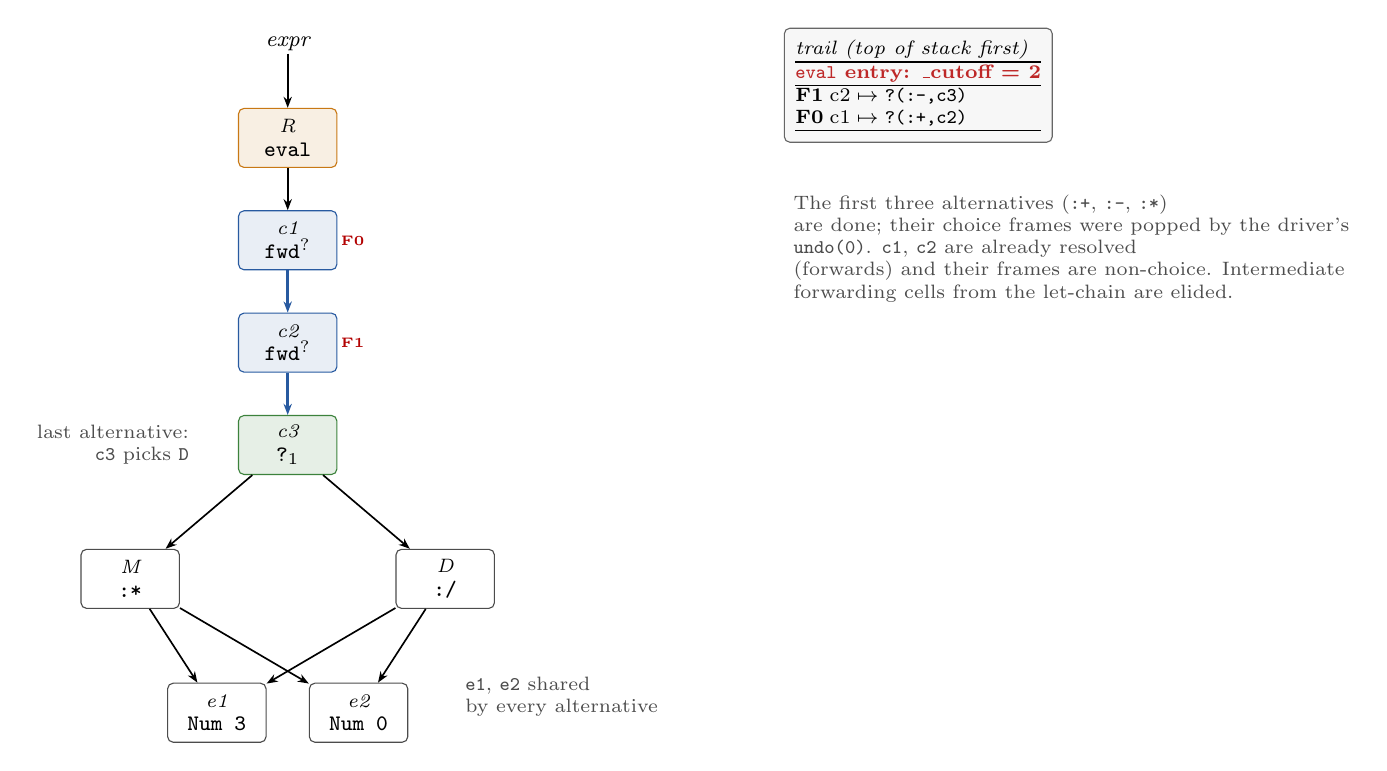
\begin{tikzpicture}
  \node[drv] (x) at (0,4.7) {expr};
  \node[fn] (R) at (0,3.5) {\cn{R}{eval}};
  \node[fw, label={[badge]right:F0}] (c1) at (0,2.2) {\cn{c1}{fwd$^?$}};
  \node[fw, label={[badge]right:F1}] (c2) at (0,0.9) {\cn{c2}{fwd$^?$}};
  \node[ch] (c3) at (0,-0.4) {\cn{c3}{?$_1$}};
  \node[co] (M) at (-2.0,-2.1) {\cn{M}{:*}};
  \node[co] (D) at (2.0,-2.1) {\cn{D}{:/}};
  \node[co] (e1) at (-0.9,-3.8) {\cn{e1}{Num 3}};
  \node[co] (e2) at (0.9,-3.8) {\cn{e2}{Num 0}};
  \draw[ptr] (x) -- (R);
  \draw[ptr] (R) -- (c1);
  \draw[fptr] (c1) -- (c2);
  \draw[fptr] (c2) -- (c3);
  \draw[ptr] (c3) -- (M);
  \draw[ptr] (c3) -- (D);
  \draw[ptr] (M) -- (e1);
  \draw[ptr] (M) -- (e2);
  \draw[ptr] (D) -- (e1);
  \draw[ptr] (D) -- (e2);
  \node[note, right=0.6 of e2, yshift=0.2cm] {\code{e1}, \code{e2} shared\\ by every alternative};
  \node[note, left=0.5 of c3, align=right] {last alternative:\\ \code{c3} picks \code{D}};
  \trailnode{6.3,4.9}{%
    \cutrow{\code{eval} entry: \_cutoff = 2}
    \fr{F1}{c2}{?(:-,c3)}{}
    \fr{F0}{c1}{?(:+,c2)}{}}
  \node[note, anchor=north west] at (6.3,2.9) {%
    The first three alternatives (\code{:+}, \code{:-}, \code{:*})\\
    are done; their choice frames were popped by the driver's\\
    \code{undo(0)}. \code{c1}, \code{c2} are already resolved\\
    (forwards) and their frames are non-choice. Intermediate\\
    forwarding cells from the let-chain are elided.};
\end{tikzpicture}
\caption{Start of the fourth and last attempt. \code{R} is the top-level
  \code{eval} node, shared by the driver's \code{expr} and, later, by trail
  frames. \code{c1}, \code{c2} were resolved to their right alternatives on
  earlier attempts. \code{c3} is the last live choice; \code{eval}
  is about to force it.}
\label{fig:a0}
\end{figure}

\begin{figure}[p]
\centering
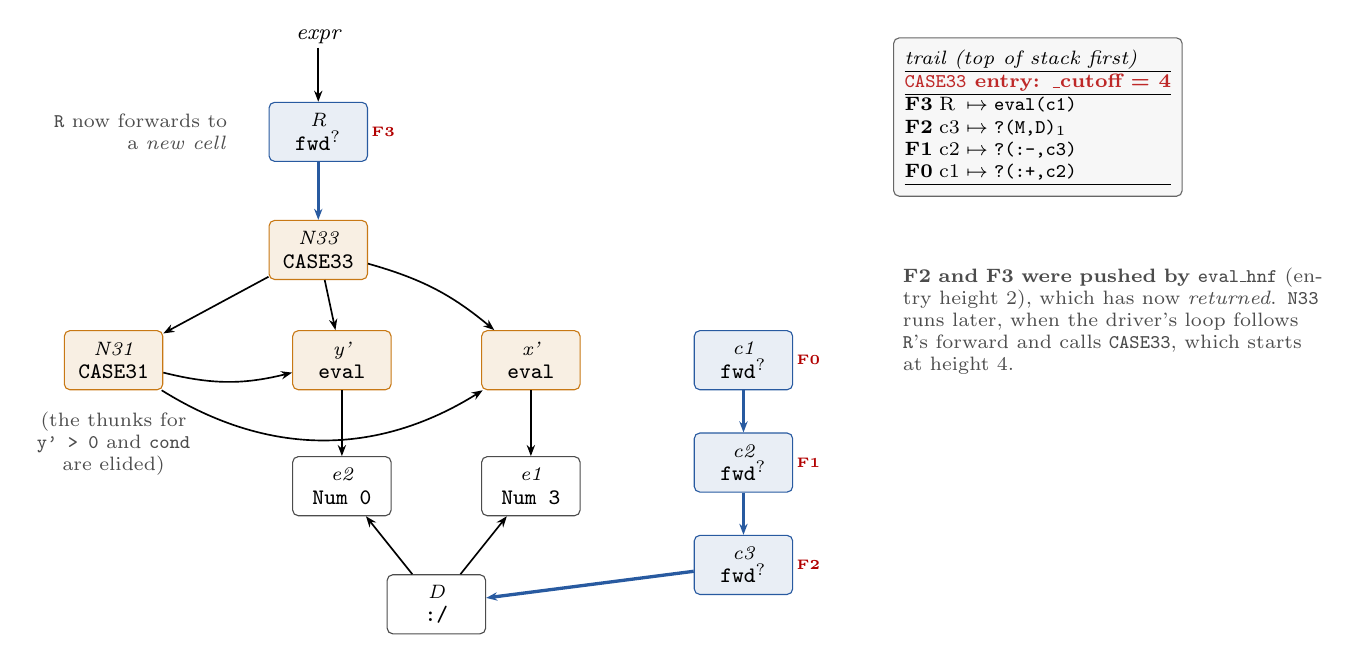
\begin{tikzpicture}
  \node[drv] (x) at (0,7.0) {expr};
  \node[fw, label={[badge]right:F3}] (R) at (0,5.8) {\cn{R}{fwd$^?$}};
  \node[fn] (N33) at (0,4.3) {\cn{N33}{CASE33}};
  \node[fn] (N31) at (-2.6,2.9) {\cn{N31}{CASE31}};
  \node[fn] (y) at (0.3,2.9) {\cn{y'}{eval}};
  \node[fn] (xx) at (2.7,2.9) {\cn{x'}{eval}};
  \node[co] (e2) at (0.3,1.3) {\cn{e2}{Num 0}};
  \node[co] (e1) at (2.7,1.3) {\cn{e1}{Num 3}};
  \node[co] (D) at (1.5,-0.2) {\cn{D}{:/}};
  \node[fw, label={[badge]right:F0}] (c1) at (5.4,2.9) {\cn{c1}{fwd$^?$}};
  \node[fw, label={[badge]right:F1}] (c2) at (5.4,1.6) {\cn{c2}{fwd$^?$}};
  \node[fw, label={[badge]right:F2}] (c3) at (5.4,0.3) {\cn{c3}{fwd$^?$}};
  \draw[ptr] (x) -- (R);
  \draw[fptr] (R) -- (N33);
  \draw[ptr] (N33) -- (N31);
  \draw[ptr] (N33) -- (y);
  \draw[ptr] (N33) to[bend left=12] (xx);
  \draw[ptr] (N31) to[bend right=14] (y);
  \draw[ptr] (N31) to[bend right=32] (xx);
  \draw[ptr] (y) -- (e2);
  \draw[ptr] (xx) -- (e1);
  \draw[ptr] (D) -- (e1);
  \draw[ptr] (D) -- (e2);
  \draw[fptr] (c1) -- (c2);
  \draw[fptr] (c2) -- (c3);
  \draw[fptr] (c3) -- (D);
  \node[note, left=0.4 of R, align=right] {\code{R} now forwards to\\ a \emph{new cell}};
  \node[note, below=0.15 of N31, align=center] {(the thunks for\\ \code{y' > 0} and \code{cond}\\ are elided)};
  \trailnode{7.3,7.0}{%
    \cutrow{\code{CASE33} entry: \_cutoff = 4}
    \fr{F3}{R}{eval(c1)}{}
    \fr{F2}{c3}{?(M,D)$_1$}{}
    \fr{F1}{c2}{?(:-,c3)}{}
    \fr{F0}{c1}{?(:+,c2)}{}}
  \node[note, anchor=north west, text width=5.4cm] at (7.3,4.2) {%
    \textbf{F2 and F3 were pushed by \code{eval\_hnf}} (entry height 2), which
    has now \emph{returned}. \code{N33} runs later, when the driver's loop
    follows \code{R}'s forward and calls \code{CASE33}, which starts at
    height 4.};
\end{tikzpicture}
\caption{\code{eval\_hnf(R)} has finished. It pushed \code{F2} (\code{c3}
  narrowed to \code{D}) and \code{F3} (\code{R}'s pre-image), rewrote
  \code{R} through a chain of tail calls, and ended with
  \code{collapse(R, N33)}: \code{R} now \emph{forwards} to a fresh cell
  \code{N33 = CASE33(N31, y', x')}. The remaining work (\code{N33}) lives in a
  different cell from the one whose pre-image the trail holds. \code{y'} and
  \code{x'} are shared by \code{N33} and by the elided thunks under
  \code{N31}. The driver then calls \code{CASE33\_hnf(N33)}, which takes its
  own \code{\_cutoff = size(bt\_stack) = 4}: the top of the stack, above
  \code{F3}.}
\label{fig:a1}
\end{figure}

\begin{figure}[p]
\centering
\textbf{(i) as generated: \code{CASE33} finds \code{N31 = False}, no \code{False} branch, calls \code{undo(4)}.}\par\smallskip
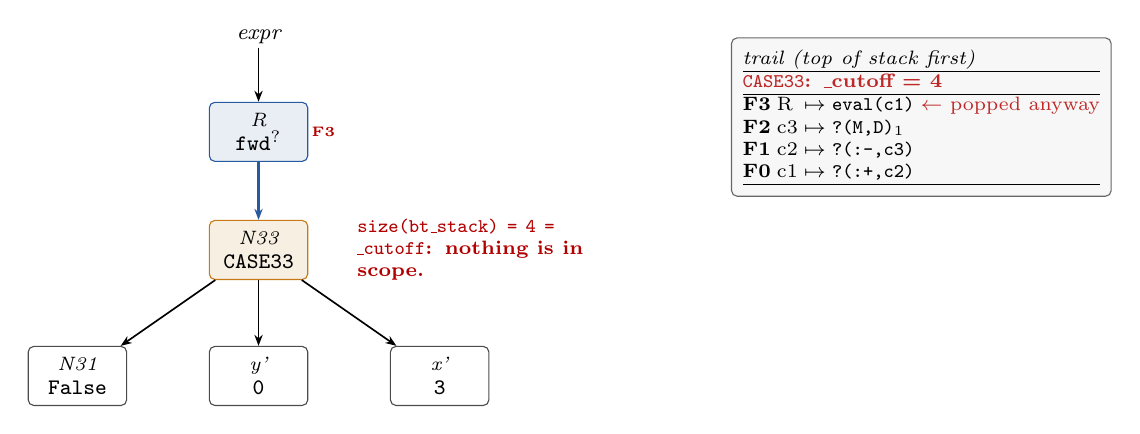
\begin{tikzpicture}
  \node[drv] (x) at (0,3.9) {expr};
  \node[fw, label={[badge]right:F3}] (R) at (0,2.7) {\cn{R}{fwd$^?$}};
  \node[fn] (N33) at (0,1.2) {\cn{N33}{CASE33}};
  \node[co] (N31) at (-2.3,-0.4) {\cn{N31}{False}};
  \node[co] (y) at (0,-0.4) {\cn{y'}{0}};
  \node[co] (xx) at (2.3,-0.4) {\cn{x'}{3}};
  \draw[ptr] (x) -- (R);
  \draw[fptr] (R) -- (N33);
  \draw[ptr] (N33) -- (N31);
  \draw[ptr] (N33) -- (y);
  \draw[ptr] (N33) -- (xx);
  \node[alarm, right=0.5 of N33, align=left] {\code{size(bt\_stack) = 4 = \_cutoff}: nothing is in scope.};
  \trailnode{6.0,3.9}{%
    \cutrow{\code{CASE33}: \_cutoff = 4}
    \fr{F3}{R}{eval(c1)}{\textcolor{cutcol}{$\leftarrow$ popped anyway}}
    \fr{F2}{c3}{?(M,D)$_1$}{}
    \fr{F1}{c2}{?(:-,c3)}{}
    \fr{F0}{c1}{?(:+,c2)}{}}
\end{tikzpicture}

\bigskip
\textbf{(ii) after \code{undo(4)} returned false and \code{fail(N33)} ran.}\par\smallskip
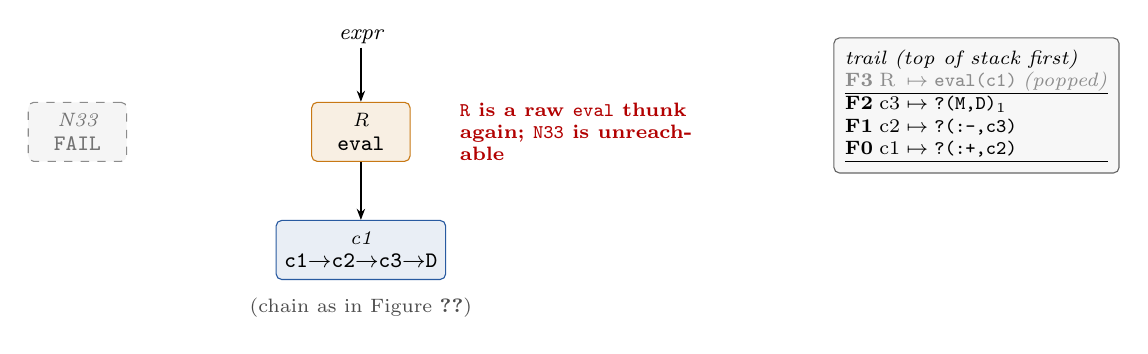
\begin{tikzpicture}
  \node[drv] (x) at (0,3.9) {expr};
  \node[fn] (R) at (0,2.7) {\cn{R}{eval}};
  \node[fw] (c1) at (0,1.2) {\cn{c1}{c1$\to$c2$\to$c3$\to$D}};
  \node[orph] (N33) at (-3.6,2.7) {\cn{N33}{FAIL}};
  \draw[ptr] (x) -- (R);
  \draw[ptr] (R) -- (c1);
  \node[alarm, right=0.5 of R, align=left] {\code{R} is a raw \code{eval} thunk again; \code{N33} is unreachable};
  \node[note, below=0.1 of c1, align=center] {(chain as in Figure~\ref{fig:a1})};
  \trailnode{6.0,3.9}{%
    \dead{F3}{R}{eval(c1)}{}
    \hline
    \fr{F2}{c3}{?(M,D)$_1$}{}
    \fr{F1}{c2}{?(:-,c3)}{}
    \fr{F0}{c1}{?(:+,c2)}{}}
\end{tikzpicture}

\bigskip
\textbf{(iii) same point if \code{undo} returns early when \code{size(bt\_stack) <= cutoff}.}\par\smallskip
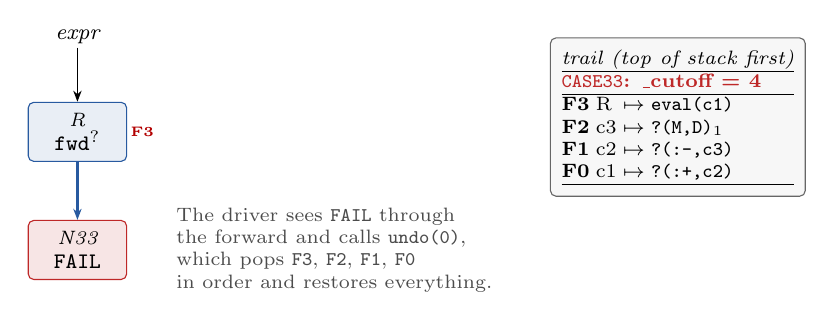
\begin{tikzpicture}
  \node[drv] (x) at (0,3.9) {expr};
  \node[fw, label={[badge]right:F3}] (R) at (0,2.7) {\cn{R}{fwd$^?$}};
  \node[fl] (N33) at (0,1.2) {\cn{N33}{FAIL}};
  \draw[ptr] (x) -- (R);
  \draw[fptr] (R) -- (N33);
  \node[note, right=0.5 of N33, align=left] {The driver sees \code{FAIL} through\\ the forward and calls \code{undo(0)},\\ which pops \code{F3}, \code{F2}, \code{F1}, \code{F0}\\ in order and restores everything.};
  \trailnode{6.0,3.9}{%
    \cutrow{\code{CASE33}: \_cutoff = 4}
    \fr{F3}{R}{eval(c1)}{}
    \fr{F2}{c3}{?(M,D)$_1$}{}
    \fr{F1}{c2}{?(:-,c3)}{}
    \fr{F0}{c1}{?(:+,c2)}{}}
\end{tikzpicture}
\caption{Defect 1 again, from the other side. \code{F3} was pushed by
  \code{eval\_hnf} before it handed off to \code{N33}, so it sits \emph{below}
  \code{CASE33}'s cutoff: \code{CASE33}'s scope is empty. \code{undo(4)} pops
  it anyway, restoring \code{R} to the raw thunk \code{eval(c1)}, which
  severs \code{R}'s forward to \code{N33}. The frame was not a choice frame,
  so \code{undo} returns false and \code{CASE33} falls through to
  \code{fail(N33)}, which marks a cell nobody points to any more. The driver
  looks at \code{expr}, finds a non-\code{FAIL} node, and prints it as a
  solution. (iii) With the guard, \code{CASE33} leaves the stack alone and
  falls through to today's unconditional \code{fail}. The driver sees
  \code{FAIL} through the forward and \code{undo(0)} pops \code{F3},
  \code{F2}, \code{F1}, \code{F0} in order, restoring everything: the same
  behavior as with scoped retry off.}
\label{fig:a2}
\end{figure}



%% ==========================================================================
\clearpage
\section{What the two failures have in common}\label{sec:summary}
%% ==========================================================================

\subsection{The invariant that breaks}

Undo is only correct if, at every moment, the trail contains a frame for
every cell that has been overwritten since the choice point being backtracked
to. Global \code{undo(0)} preserves this trivially: it empties the log, so
nothing is left to disagree with. \emph{A scoped undo removes a suffix of the
log and then keeps executing}, so the invariant has to hold for the frames it
\emph{leaves} as well as the ones it removes. Both defects break it:

\begin{description}[leftmargin=1.5em, style=nextline]
\item[Defect 1: \code{undo} pops a frame outside its scope.]
  The \code{do}/\code{while} pops once before testing \code{size >
  cutoff}. If the scope is empty (\code{size == cutoff}) it removes a
  frame that belongs to an ancestor computation and restores that
  ancestor's cell. Figures~\ref{fig:b3} and~\ref{fig:a2}. In
  Example~2 the ancestor is \code{eval\_hnf}: the trail is address-keyed and
  \code{R}'s pre-image is just ``a frame'', with nothing to say it belongs to
  a computation whose continuation lives in another cell.
\item[Defect 2: a failed retry leaves \code{root} mutated without a frame.]
  In an \code{IExempt} branch the emitter (\code{ToC.curry},
  \code{showConsBranch}~$+$~\code{showStmt ctx n IExempt}) writes
  \code{save\_copy(root); SCOPED\_RETRY; fail(root)}. An unsuccessful retry
  pops the frame \code{save\_copy} just pushed, so \code{fail(root)}
  mutates \code{root} unlogged, and restoring the pre-image also resets
  \code{root}'s \code{nondet} bit to its earlier value (false in
  Figure~\ref{fig:b2}). The \code{FAIL\_TAG} path is
  emitted in the right order and does not have this problem.
\end{description}

\subsection{Where sharing comes in}

\begin{itemize}[nosep]
\item \textbf{Why there is a log at all.} Every parent of a shared cell sees
  its in-place update. \code{R} is shared between the driver and the trail;
  \code{G} and \code{c} are shared between two branches of the same call.
  Undo has to restore cells \emph{by address}, whichever parent asks.
\item \textbf{Why the log cannot tell whose entry it is.} Frames are
  \code{cell $\mapsto$ pre-image}. They carry no record of which function
  pushed them. \code{\_cutoff} is a stack height, an approximation of
  ``mine''. It is exact only while a function's whole computation stays
  inside one C activation. \code{TAIL\_DISPATCH} and \code{collapse} break
  that: control moves along a heap edge (\code{R} $\to$ \code{N33}) or into a
  sibling function (\code{CASE7}), and the callee's height sits \emph{above}
  its logical parent's frames.
\item \textbf{Why a shared choice makes the failure non-local.} In Example 1
  the choice \code{c} is made by \code{F}'s dispatch, but the failure it
  causes is found inside \code{G}. \code{c}'s frame is below \code{G}'s
  cutoff, so \code{G} cannot retry it. The only correct move is to fail
  \emph{and say why}: leave a frame that restores \code{G} and keep
  \code{G}'s \code{nondet} bit, so that \code{F} logs itself and global
  backtracking can revisit \code{c}. Defect 2 destroys exactly that
  information.
\end{itemize}

\subsection{What I ran}

Every variant below was built in a scratch directory from the current tree:
\code{-DOPT\_SCOPED\_BACKTRACK=0} for ``off''; the tree as is for ``on'';
\emph{guard} is a one-line change to a scratch copy of \code{undo} (return
false if \code{size(bt\_stack) <= cutoff}); \emph{re-save} is a text patch to
the generated C (and to \code{Prelude.c}) that inserts
\code{if(nondet) save\_copy(root);} between \code{SCOPED\_RETRY} and
\code{fail(root)} in the \code{IExempt} path. No source file in the repository was edited; the only additions are this note and its PDF.

\begin{table}[htb]
\centering
\small
\begin{tabular}{@{}lccccc@{}}
\toprule
& off & on (default) & guard only & re-save only & guard + re-save \\
\midrule
Example 1 (\code{nested}) & ok & \textbf{lost \code{2}} & \textbf{lost \code{2}} & ok & ok \\
Example 2 (\code{cent\_tiny}) & ok & \textbf{prints raw \code{eval(\ldots)}} & ok & --- & ok \\
\code{cent} (528 solutions) & ok & \textbf{1133 distinct} & ok & --- & ok \\
\bottomrule
\end{tabular}
\caption{``ok'' means the real solutions match scoped retry off (for
  \code{cent}: exactly the 528 lines of \code{cent.expected}, after dropping
  \code{SOLUTION: FAIL} lines, see below). ``---'' means not run. The
  default build's 1133 distinct solutions for \code{cent} are 404 correct plus
  729 that do not evaluate to the target, matching \code{current.md}.}
\label{tab:runs}
\end{table}

\subsection{What this does and doesn't show}

\begin{itemize}[nosep]
\item Fixing defect 1 alone is enough for \code{cent\_tiny} and \code{cent};
  fixing defect 2 alone is enough for \code{nested} (Table~\ref{tab:runs}).
  Defect 1 also fires in \code{nested} (Figure~\ref{fig:b3}) but is
  harmless there once defect 2 is fixed, because the \code{FAIL\_TAG}
  path re-saves \code{root}.
\item Neither patch has been run against \code{tests/run.sh}, so this is
  evidence that the two defects are \emph{sufficient} for these failures,
  not that scoped retry is now sound. I have not tried to construct a
  program where defect 1 pops a \emph{choice} frame (the case noted in the
  caption of Figure~\ref{fig:b3}), and I have not argued about ICaseLit or
  the free-variable path.
\item Even with both patches, a retry in \code{CASE33} can never reach a
  choice made by \code{eval\_hnf}: those frames are below \code{CASE33}'s
  cutoff (here \code{c3} has no alternative left anyway). Scoped retry stays
  a strictly local optimization; recovering such cases would need the cutoff to be inherited
  across \code{collapse}/\code{TAIL\_DISPATCH} edges, and then the retry
  would also have to redo the \emph{dispatch} that depended on the choice,
  not just re-read the scrutinee.
\item \code{tests/run.sh --slow cent} currently reports an output mismatch
  for the default build: the golden file has no \code{SOLUTION: FAIL} lines,
  while every build I made, including scoped retry off, prints them (\code{nf\_all}
  prints a solution unless \code{TAG(expr) == FAIL\_TAG}; in the traces
  \code{expr} is a forward to a \code{FAIL} cell). This is independent of scoped retry and
  contradicts \code{current.md}'s note that the suite passes; I have not
  chased it further.
\end{itemize}

\end{document}
